\begin{frame}{Diagrama de señales entre la Interfaz USB y el FPGA}
	\centering
	\begin{tikzpicture}[scale=.7]
		\begin{scope}[transform shape,node distance=4,>=latex,double distance=1.3]
			\node[simple](mef)[]{Maquina de Estados Finitos};
			\node[simple] (fifo) [left=of mef] {FIFO Esclava\\Controlador FX2LP};			

			\node[simple,minimum width=85](interno)[right=of mef]{Sistema\\Implementado en FPGA};
			\draw[double,->]([yshift=5*220/8]mef.south east)--node[above](rec){Dato\_recibido[15:0]} ([yshift=5*220/8]interno.south west);
			\draw[double,<-]([yshift=4*220/8]mef.south east)--node[above](aEnv){Dato\_a\_enviar[15:0]}([yshift=4*220/8]interno.south west);
			\draw[<-]([yshift=3*220/8]mef.south east)--node[above](env){Enviar\_datos}([yshift=3*220/8]interno.south west);
			\draw[->]([yshift=2*220/8]mef.south east)--node[above](intrd){SLRD}([yshift=2*220/8]interno.south west);
			\draw[->]([yshift=1*220/8]mef.south east)--node[above](intwr){SLWR}([yshift=1*220/8]interno.south west);	
			\draw[<-]([yshift=-1*220/8]mef.north east)--node[above](clk){Reloj}([yshift=-1*220/8]interno.north west);
			\draw[<-]([yshift=-2*220/8]mef.north east)--node[above](rst){Reset}([yshift=-2*220/8]interno.north west);

			\draw[<->,thick] ([yshift=5*110/6]fifo.east) --node [above](ifclk){IFCLK} ([yshift=5*110/6]mef.west);
			\draw[<->,thick]	([yshift=4*110/6]fifo.east) --node [above](fd){FD[15:0]} ([yshift=4*110/6]mef.west);
			\draw[<-,thick]	([yshift=3*110/6]fifo.east) --node [above](fifoadr){FIFOADR[1:0]} ([yshift=3*110/6]mef.west);
			\draw[->,thick]	([yshift=2*110/6]fifo.east) --node [above](flaga){FLAGA} ([yshift=2*110/6]mef.west);
			\draw[->,thick]	([yshift=1*110/6]fifo.east) --node [above](flagb){FLAGB} ([yshift=1*110/6]mef.west);
			\draw[->,thick]	([yshift=0*110/6]fifo.east) --node [above](flagc){FLAGC} ([yshift=0*110/6]mef.west);
			\draw[->,thick]	([yshift=-1*110/6]fifo.east) --node [above](flagd){FLAGD} ([yshift=-1*110/6]mef.west);
			\draw[<-,thick]	([yshift=-2*110/6]fifo.east) --node [above](sloe){SLOE} ([yshift=-2*110/6]mef.west);
			\draw[<-,thick]	([yshift=-3*110/6]fifo.east) --node [above](slwr){SLWR} ([yshift=-3*110/6]mef.west);
			\draw[<-,thick]	([yshift=-4*110/6]fifo.east) --node [above](slrd){SLRD} ([yshift=-4*110/6]mef.west);
			\draw[<-,thick]	([yshift=-5*110/6]fifo.east) --node [above](pktend){PKTEND} ([yshift=-5*110/6]mef.west);
		\end{scope}
		\begin{scope}[]
			\node[draw=blue,dashed,rectangle,fit={(mef)(interno)},label=north:FPGA,rounded corners]{};
			\action<2>{\node[ultra thick,draw=blue,ellipse,fit=(fd)] {};}
			\action<3>{\node[ultra thick,draw=blue,ellipse,fit=(fifoadr)] {};}
			\action<4>{\node[ultra thick,draw=blue,ellipse,fit=(flaga)(flagb)] {};}
			\action<5>{\node[ultra thick,draw=blue,ellipse,fit=(sloe)] {};}
			\action<5>{\node[ultra thick,draw=blue,ellipse,fit=(slrd)] {};}
			\action<6>{\node[ultra thick,draw=blue,ellipse,fit=(slwr)] {};}
			\action<7>{\node[ultra thick,draw=blue,ellipse,fit=(pktend)] {};}
			\action<8>{\node[ultra thick,draw=blue,ellipse,fit=(clk)(rst)] {};}
			\action<9>{\node[ultra thick,draw=blue,ellipse,fit=(rec)] {};}
			\action<10>{\node[ultra thick,draw=blue,ellipse,fit=(aEnv)] {};}
			\action<11>{\node[ultra thick,draw=blue,ellipse,fit=(env)] {};}
			\action<12>{\node[ultra thick,draw=blue,ellipse,fit=(intrd)] {};}
			\action<13>{\node[ultra thick,draw=blue,ellipse,fit=(intwr)] {};}
		\end{scope}
	\end{tikzpicture}
\end{frame}

\begin{frame}{Operaciones en la FIFO}
	\framesubtitle{Escritura Asíncrona}
	\centering
	\begin{tikzpicture}[scale=.85,text width=50,align=center,transform shape]
		\node[exterior,rounded corners](fx2lp){Interfaz\\USB};
		\node[exterior,rounded corners](fpga)[right=of fx2lp]{FPGA};
		\draw[->,blue,ultra thick](fpga)to(fx2lp);
	\end{tikzpicture}
	\begin{tikzpicture}[scale=.85]
		\begin{scope}[transform shape,node distance=1,text width=60]
			\setcounter{wavecount}{0}
			\newwave{FIFOADR[1]}
				\bit{0}{9}
			\newwave{FIFOADR[0]}
				\bit{0}{9}
			\newwave{FLAG\_Lleno}
				\only<-7>{
					\bit{1}{6}
					\bit{0}{3}}
				\only<8->{
					\bit{1}{4}
					\bit{0}{5}
				}
			\newwave{SLWR}
				\only<-7>{
					\bit{1}{3}
					\bit{0}{1}
					\bit{1}{1}
					\bit{0}{1}
					\bit{1}{1}
					\bit{0}{1}
					\bit{1}{1}
				}
				\only<8->{
					\bit{1}{3}
					\bit{0}{1}
					\bit{1}{1}
					\bit{0}{1}
					\bit{1}{1}
					\bit{0}{1}
					\bit{1}{1}
				}
			\newwave{PKTEND}
				\only<-7>{
					\bit{1}{9}
				}
				\only<8->{
					\bit{1}{3}
					\bit{0}{1}
					\bit{1}{5}
				}
			\newwave{FD[15:0]}
				\only<-7>{
				\bitvector{N-2}{3}
				\bitvector{N-1}{2}
				\bitvector{N}{2}
				\graybitvector{No leído}{2}	
				}
				\only<8->{
					\bitvector{N-20}{3}
					\bitvector{N-19}{2}
					\graybitvector{No leído}{4}
				}
			\action<2>{\draw[blue, ultra thick] (0.3,-0.6) ellipse (.6 and 1.2);}
			\action<3-5>{\draw[blue, ultra thick] (3.3,-3) ellipse (.5 and .6);}
			\action<4-5>{\draw[blue, ultra thick] (3.3,-5) ellipse (.5 and .6);}
			\action<5-6>{\draw[blue, ultra thick] (5.3,-3) ellipse (.5 and .6);}
			\action<5-6>{\draw[blue, ultra thick] (5.3,-5) ellipse (.5 and .6);}
			\action<6-7>{\draw[blue, ultra thick] (6.3,-2) ellipse (.5 and .6);}
			\action<7>{\draw[blue, ultra thick] (7.3,-3) ellipse (.5 and .6);}
			\action<7>{\draw[red, ultra thick] (8.3,-5) ellipse (1 and .6);}
			\action<9->{\draw[blue,ultra thick](3.3,-4)ellipse(.5 and .6);}
			\action<10->{\draw[blue,ultra thick](4.3,-2)ellipse(.5 and .6);}
			\action<10->{\draw[red,ultra thick](7.3,-5)ellipse(2 and .6);}
		\end{scope}
		\begin{scope}[on background layer]
			\foreach \x in {1,2,...,9}{
				\draw[dashed,black!20] (\x.3,0) -- (\x.3,\value{wavecount}+1);}
		\end{scope}
	\end{tikzpicture}
\end{frame}

\begin{frame}{Operaciones en la FIFO}
	\framesubtitle{Lectura Asíncrona}
	\centering
	\begin{tikzpicture}[scale=.85,text width=50,align=center,transform shape]
		\node[exterior,rounded corners](fx2lp){Interfaz\\USB};
		\node[exterior,rounded corners](fpga)[right=of fx2lp]{FPGA};
		\draw[<-,blue,ultra thick](fpga)to(fx2lp);
	\end{tikzpicture}
	\begin{tikzpicture}[scale=.85]
		\begin{scope}[transform shape,node distance=1,text width=60]
			\setcounter{wavecount}{0}
			\newwave{FIFOADR[1]}
				\bit{1}{9}
			\newwave{FIFOADR[0]}
				\bit{1}{9}
			\newwave{FLAG\_Vac\'io}
				\bit{1}{5}
				\bit{0}{4}
			\newwave{SLOE}
				\bit{1}{1}
				\bit{0}{7}
				\bit{1}{1}
			\newwave{SLRD}
				\bit{1}{2}
				\bit{0}{1}
				\bit{1}{1}
				\bit{0}{1}
				\bit{1}{1}
				\bit{0}{1}
				\bit{1}{2}
			\newwave{FD[15:0]}
				\bitvector{Z}{1}
				\bitvector{N-1}{2}
				\bitvector{N}{2}
				\graybitvector{No válido}{3}
				\bitvector{Z}{1}
			\action<2>{\draw[blue,ultra thick](.3,-.5)ellipse(0.5 and 1);}
			\action<3>{\draw[blue,ultra thick](1.3,-3)ellipse(0.5 and .6);}
			\action<3>{\draw[blue,ultra thick](0.8,-5)ellipse(0.5 and .6);}
			\action<4>{\draw[blue,ultra thick](2.3,-4.5)ellipse(0.6 and 1);}
			\action<5>{\draw[blue,ultra thick](3.3,-4.5)ellipse(0.5 and 1);}
			\action<6>{\draw[blue,ultra thick](5.3,-2)ellipse(0.5 and .6);}
			\action<6>{\draw[red,ultra thick](6.8,-5)ellipse(1 and .6);}
		\end{scope}
		\begin{scope}[on background layer]
			\foreach \x in {1,2,...,9}{
				\draw[dashed,black!20] (\x.3,0) -- (\x.3,\value{wavecount}+1);}
		\end{scope}
	\end{tikzpicture}
\end{frame}

\begin{frame}{Máquina de estados algorítmica sintetizada en FPGA}
	\centering
	\begin{tikzpicture}[ask/.style = {diamond,text width=70,draw=black,align=center,aspect=2},
	scale=.41]
		\begin{scope}[transform shape,node distance=(1 and 4),>=latex,]
			\node[moore,text width=110] (inicio) [label=above right:inicio]{FIFOADR=$''$ZZ$''$\\FDATA=$''$ZZ$''$\\d\_recibido=d\_recibido\\SLOE=$'1'$\\SLRD=$'1'$\\SLWR=$'1'$};
		
			\node[ask] (vacio1) [below=of inicio]{FLAG\_Vacío};
				\draw[->] (inicio.south) -| (vacio1);
		
			\node[moore,text width=110] (lecoe) [right=of vacio1,label=above right:dir\_lect] {FIFOADR=$''11''$\\FDATA=$''$ZZ$''$\\d\_recibido=FD\\SLOE=$'0'$\\SLRD=$'1'$\\SLWR=$'1'$};
				\draw[->] (vacio1.east) -- ($(vacio1.east)!0.5!(lecoe.west)$);
				\draw[->]($(vacio1.east)!0.5!(lecoe.west)$) |- ($(lecoe.north)+(0,1)$) -- (lecoe.north);
		
			\node[moore,text width=110](lecrd)[below=of lecoe,label=above right:lectura]{FIFOADR=$''11''$\\FDATA=$''$ZZ$''$\\D\_recibido=FD\\SLOE=$'0'$\\SLRD=$'0'$\\SLWR=$'1'$};
				\draw[->](lecoe) -- (lecrd);
		
			\node[ask] (vacio2)[below=of lecrd]{FLAG\_Vacío};
				\draw[->](lecrd) -- (vacio2);
				
				\draw[->](vacio2.west) -| ($(lecoe.west)!.5!(vacio1.east)$);
				\draw[o->](vacio2.east) -- ++(1.5,0) |- ($(inicio.north)+(0,1)$);
				\draw[->] ($(inicio.north)+(0,1)$) -- (inicio.north);
		
			\node[ask](enviar1)[below=of vacio1]{Enviar\_datos};
				\draw[o->](vacio1.south) --(enviar1.north);
		
		
			\node[ask] (lleno1) [below=of enviar1]{FLAG\_Lleno};
				\draw[->](enviar1) -- (lleno1);
		
			\node[moore,text width=110](escdir)[below=of lleno1,label=above left:dir\_escr]{FIFOADR=$''00''$\\FDATA=d\_a\_enviar\\d\_recibido=d\_recibido\\SLOE=$'1'$\\SLRD=$'1'$\\SLWR=$'0'$};
				\draw[->](lleno1) -- ($(lleno1.south)!0.5!(escdir.north)$);
				\draw[->]($(lleno1.south)!0.5!(escdir.north)$) -- (escdir);
		
		
			\node[ask](vacio3)[left=of vacio1]{FLAG\_Vacío};
				\draw[->](escdir.south)--($(escdir.south)+(0,-.5)$) -| ($(vacio3.east)+(1,0)$) |- ($(vacio3.north)+(0,1)$)-|(vacio3.north);
		
			\node[ask](enviar2)[below=of vacio3]{Enviar\_datos};
				\draw[o->](vacio3) -- (enviar2);
		
				\draw[o->] (enviar1.west) -- ($(enviar1.west)+(-1,0)$);
				\draw[->] ($(enviar1.west)-(1,0)$) -- ($(inicio.north -| enviar1.west)+(-1,1)$);
				\draw[->] ($(inicio.north -| enviar1.west)+(-1,1)$)--($(inicio.north)+(0,1)$);
				\draw[->] ($(inicio.north)+(0,1)$) -- (inicio.north);
				\draw[o->](lleno1.west) -| ($(enviar1.west)-(1,0)$);
				\draw[->](vacio3.west) -- ($(vacio3.west)+(-1,0)$);
				\draw[->]($(vacio3.west)+(-1,0)$) |- ($(inicio.north -| enviar1.west)+(-1,1)$);
		
			\node[ask](lleno2)[below=of enviar2]{FLAG\_Lleno};
			\node[moore,text width=110](escwr)[below=of lleno2,label=above left:escribir]{FIFOADR=$''00''$\\FDATA=d\_a\_enviar\\d\_recibido=d\_recibido\\SLOE=$'1'$\\SLRD=$'1'$\\SLWR=$'1'$};
				\draw[->](lleno2) -- (escwr);
				\draw[o->](lleno2.west) -| ($(enviar2.west)+(-1,0)$);
				\draw[->](enviar2)--(lleno2);
				\draw[o->](enviar2)--($(enviar2.west)+(-1,0)$);
				\draw[->]($(enviar2.west)+(-1,0)$) -- ($(vacio3.west)+(-1,0)$);
				\draw[->](escwr) -- ($(escwr.south)+(0,-1)$) -| ($(escdir.east)+(1,0)$) |- ($(lleno1.south)!0.5!(escdir.north)$);
		\end{scope}
		\begin{scope}
			\action<2-3,7-8>{\node[ultra thick,draw=blue,ellipse,fit=(inicio)]{};}
			\action<6,11>{\node[ultra thick,draw=red,ellipse,fit=(inicio)]{};}
			\action<3,7>{\node[ultra thick,draw=red,ellipse,fit=(vacio1)]{};}
			\action<3,6>{\node[ultra thick,draw=red,ellipse,fit=(lecoe)]{};}
			\action<4>{\node[ultra thick,draw=blue,ellipse,fit=(lecoe)]{};}
			\action<5-6>{\node[ultra thick,draw=blue,ellipse,fit=(lecrd)]{};}
			\action<6>{\node[ultra thick,draw=red,ellipse,fit=(vacio2)]{};}
			\action<8>{\node[ultra thick,draw=red,ellipse,fit=(enviar1)]{};}
			\action<8>{\node[ultra thick,draw=red,ellipse,fit=(lleno1)]{};}
			\action<9-11,13>{\node[ultra thick,draw=blue,ellipse,fit=(escdir)]{};}
			\action<10>{\node[ultra thick,draw=red,ellipse,fit=(vacio3)(enviar2)(lleno2)]{};}
			\action<11>{\node[ultra thick,draw=red,ellipse,fit=(escwr)]{};}
			\action<12>{\node[ultra thick,draw=blue,ellipse,fit=(escwr)]{};}
		\end{scope}
	\end{tikzpicture}
\end{frame}

\begin{frame}{Verificación Funcional}

		\framesubtitle{Operación de lectura}
		\centering
	\begin{tikzpicture}[scale=.85,text width=50,align=center,transform shape]
		\node[exterior,rounded corners](fx2lp){Interfaz\\USB};
		\node[exterior,rounded corners](fpga)[right=of fx2lp]{FPGA};
		\draw[<-,blue,ultra thick](fpga)to(fx2lp);
	\end{tikzpicture}
		\only<1>{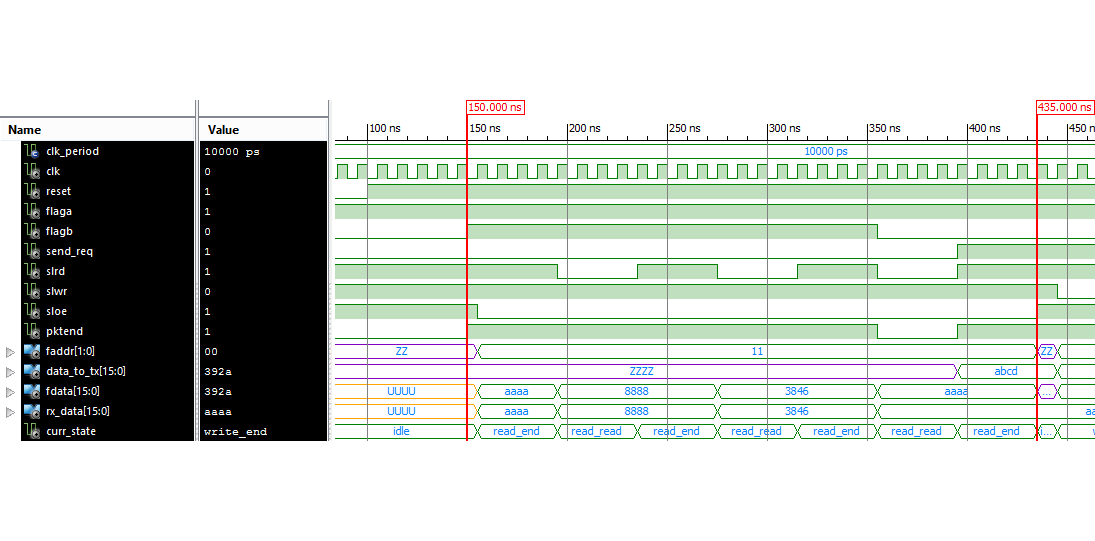
\includegraphics[width=\textwidth]{mef_tb_lect00}}
		\only<2>{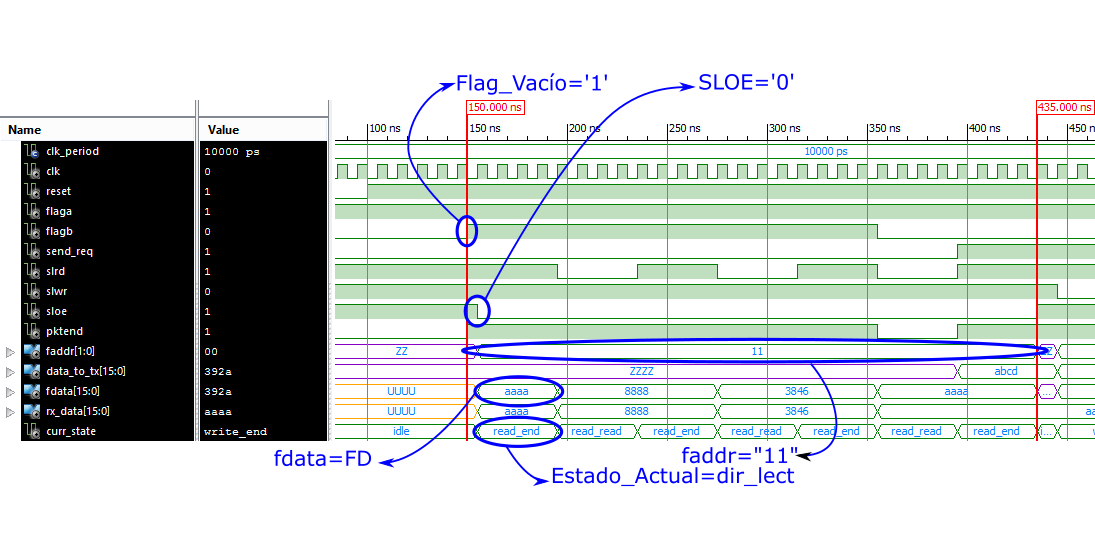
\includegraphics[width=\textwidth]{mef_tb_lect01}}
		\only<3>{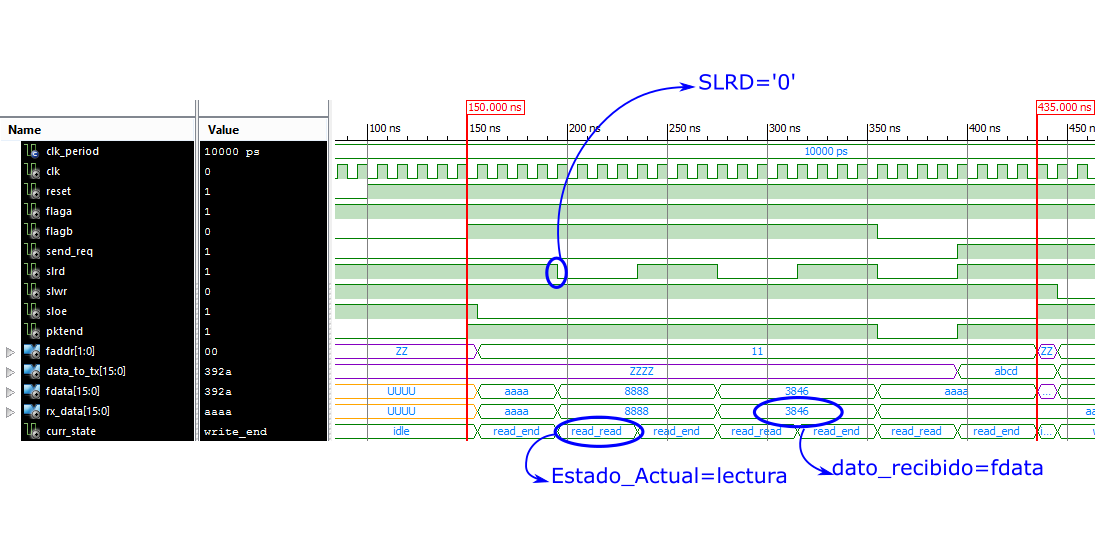
\includegraphics[width=\textwidth]{mef_tb_lect02}}
		\only<4>{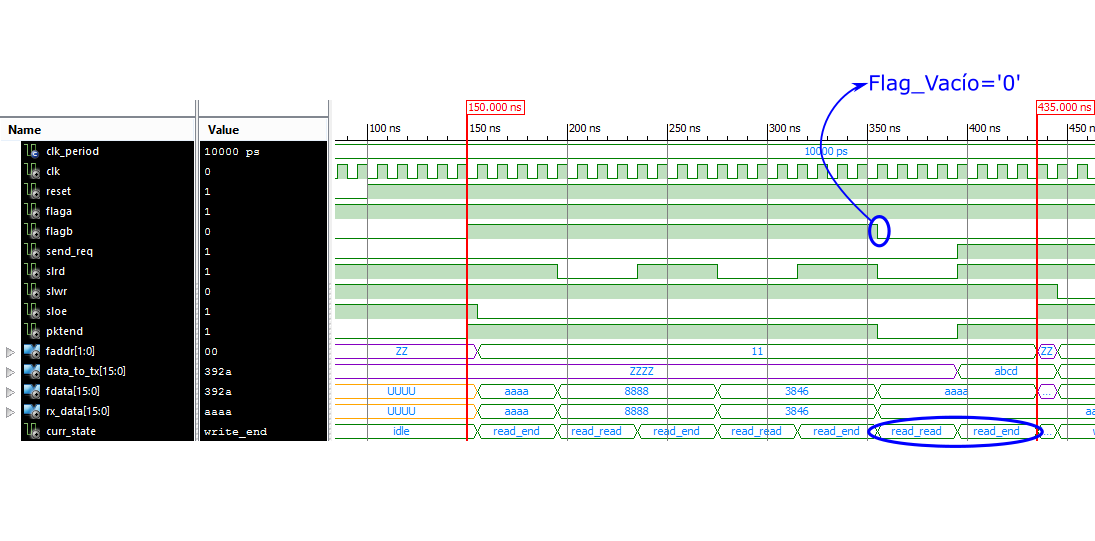
\includegraphics[width=\textwidth]{mef_tb_lect03}}
\end{frame}

\begin{frame}{Verificación Funcional}
	\framesubtitle{Operación de escritura}
	\centering
	\begin{tikzpicture}[scale=.85,text width=50,align=center,transform shape]
		\node[exterior,rounded corners](fx2lp){Interfaz\\USB};
		\node[exterior,rounded corners](fpga)[right=of fx2lp]{FPGA};
		\draw[->,blue,ultra thick](fpga)to(fx2lp);
	\end{tikzpicture}
		\only<1>{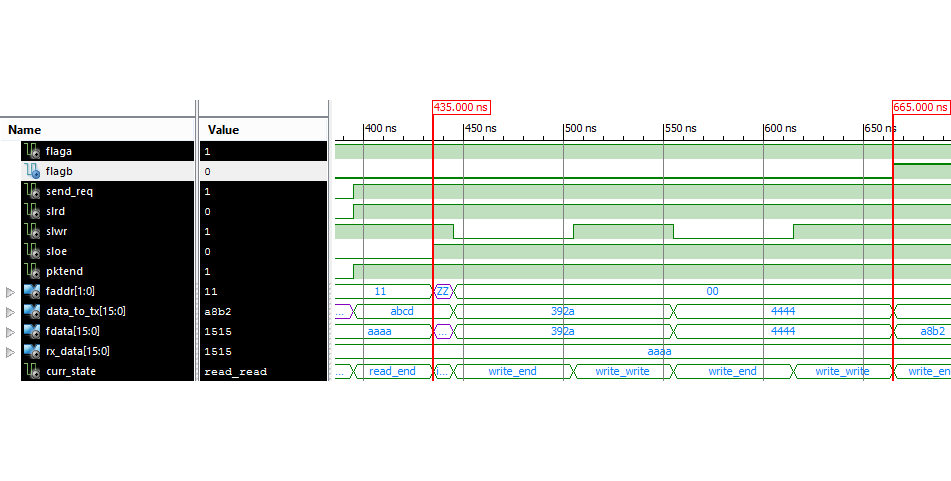
\includegraphics[width=\textwidth]{mef_tb_escr00}}
		\only<2>{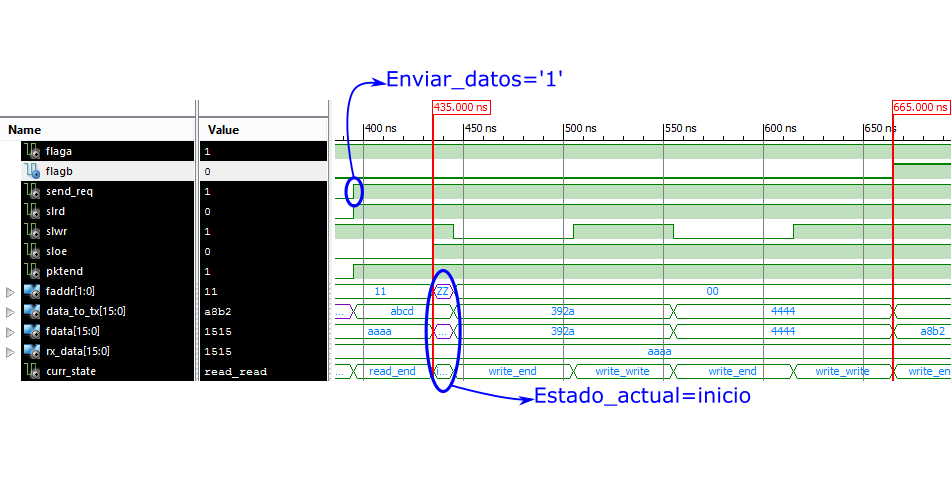
\includegraphics[width=\textwidth]{mef_tb_escr01}}
		\only<3>{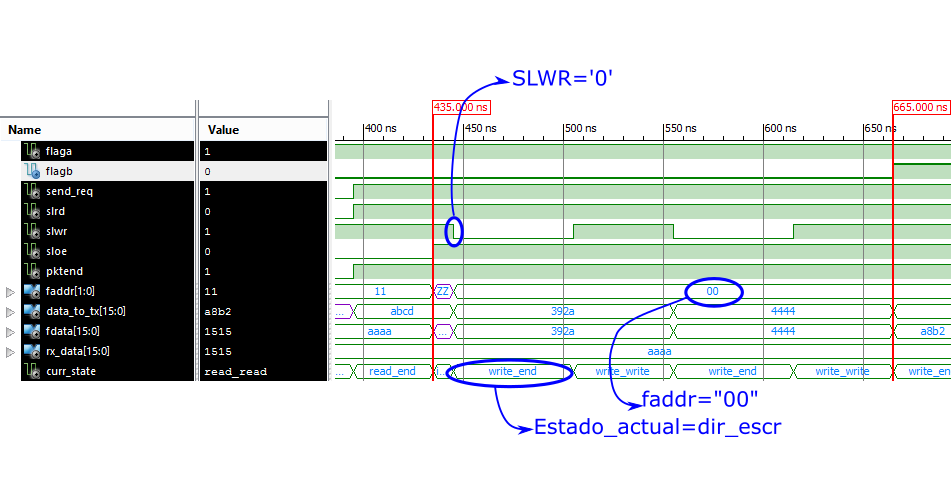
\includegraphics[width=\textwidth]{mef_tb_escr02}}
		\only<4>{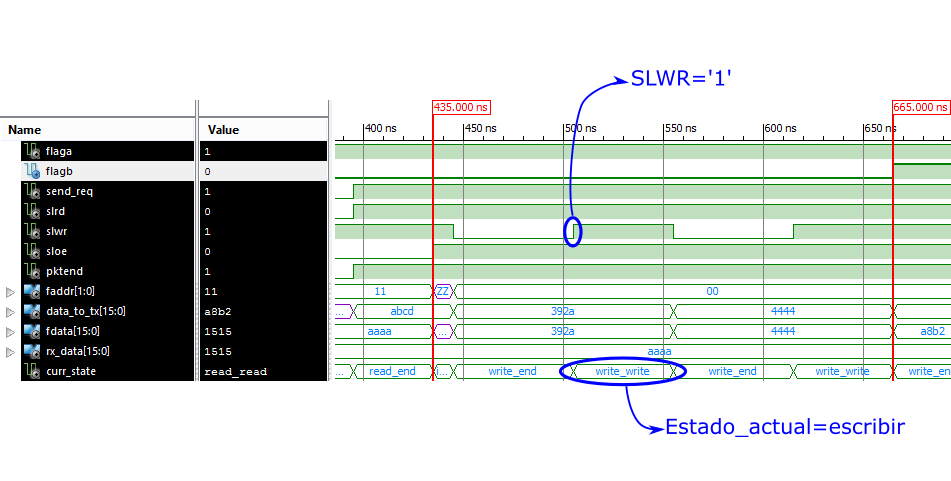
\includegraphics[width=\textwidth]{mef_tb_escr03}}

		\only<5>{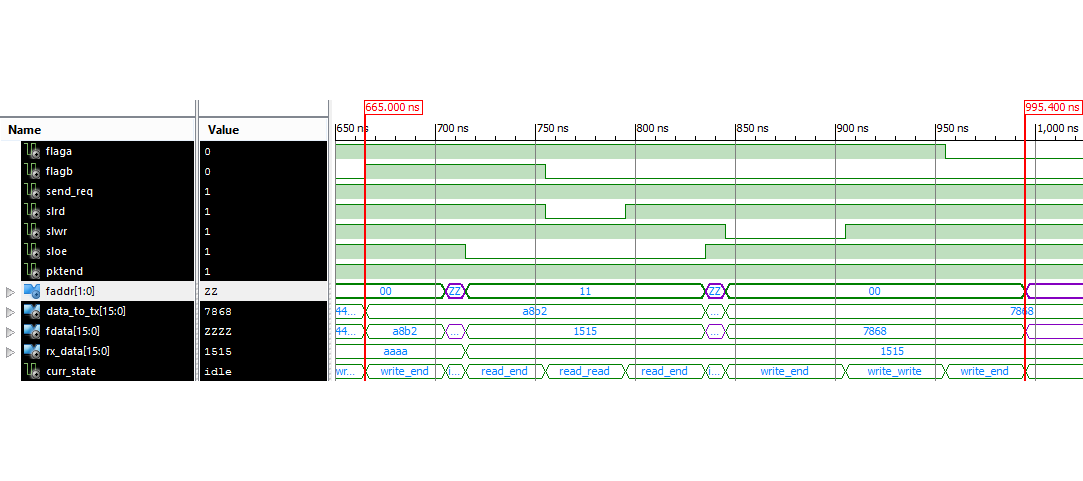
\includegraphics[width=\textwidth]{mef_tb_full00}}
		\only<6>{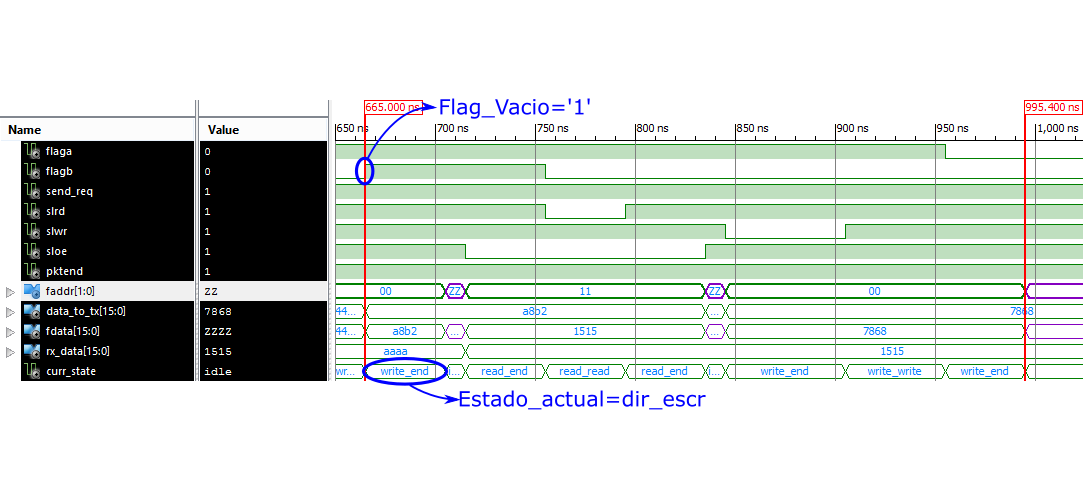
\includegraphics[width=\textwidth]{mef_tb_full01}}
		\only<7>{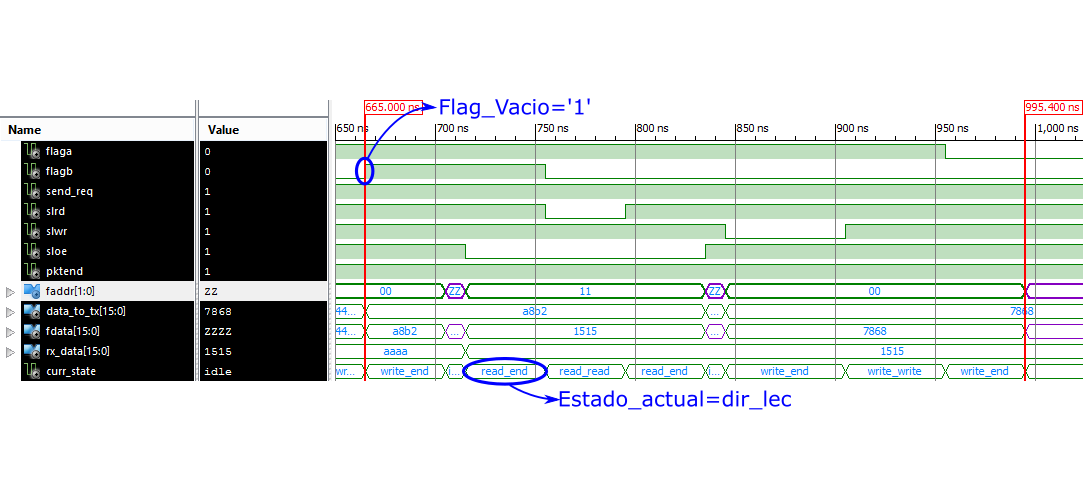
\includegraphics[width=\textwidth]{mef_tb_full02}}
		\only<8>{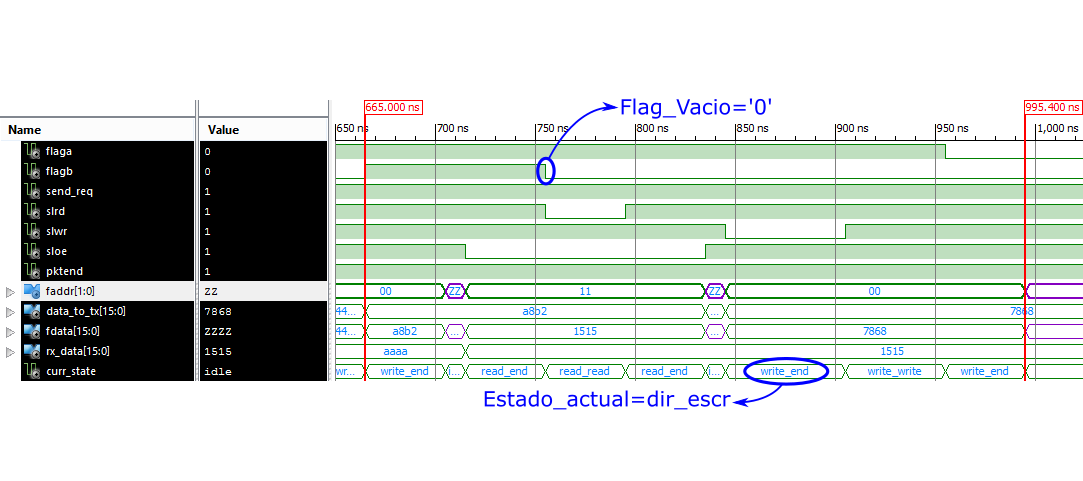
\includegraphics[width=\textwidth]{mef_tb_full03}}
		\only<9>{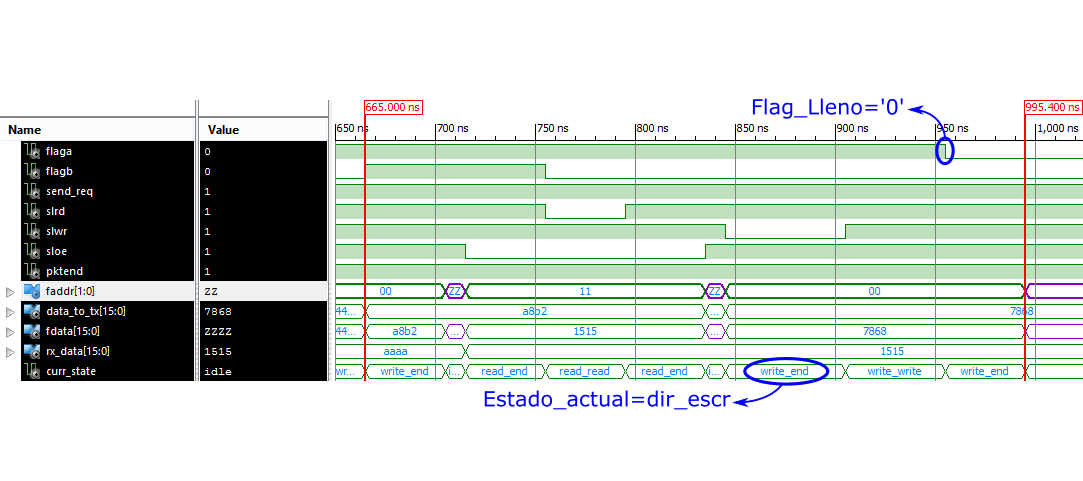
\includegraphics[width=\textwidth]{mef_tb_full04}}
\end{frame}